\documentclass[hyperref={colorlinks = true,linkcolor = blue, citecolor = blue, urlcolor = blue}]{beamer}

\setbeamertemplate{navigation symbols}{}
\setbeamertemplate{footline}[frame number]
 
\usepackage[normalem]{ulem}
\usepackage[utf8]{inputenc}

\usepackage[newfloat]{minted}

\usepackage{pgf}
\usepackage{tikz}
\usepackage{upquote}
\usepackage{natbib}
\usetikzlibrary{arrows,automata}

\bibliographystyle{abbrvnat}


\newenvironment{code}{\captionsetup{type=listing}}{}
\SetupFloatingEnvironment{listing}{name=Listing}

\title{Monoids and Monads}
\author{Donovan Crichton}
\date{August 2022}

\begin{document}
 
\frame{\titlepage}

\begin{frame}[fragile]
  \frametitle{Preliminaries}
  \begin{itemize}
  \item Slides and Examples available at:
    \url{https://github.com/donovancrichton/ANU-FP}
  \item This talk: /MonoidsAndMonads
  \end{itemize}
\end{frame}

\begin{frame}[fragile]
  \frametitle{Last Week}
  \begin{itemize}
    \item Type Classes in Haskell are almost an Algebra, Haskell has no way to express the laws.
    \item Idris lets us express the laws via proofs of equality.
    \item We saw Functor and Applicative type classes.
    \item We left some future work on the proof of Applicative laws for this week.
  \end{itemize}
\end{frame}

\begin{frame}[fragile]
  \frametitle{Functors}
  \begin{itemize}
    \item The Functor interface lets us map over a structure. Letting us transform the underlying elements into new elements.
    \item Applicative lets us apply pure functions to `funny types' \citep{mcbride2008applicative}.
  \end{itemize}
  For example:
  \begin{minted}{idris}
-- change a list of number to a list of functions.
(\x => MkPair x) <$> [1, 2, 3] : Num a => [b -> (a, b)]

-- lift a pure function up to apply to maybe types
(pure (+)) <*> (Just 2) <*> (Just 3) = Just 5
  \end{minted}
\end{frame}

\begin{frame}[fragile]
  \frametitle{Functors}
  \begin{itemize}
    \item The Functor interface lets us map over a structure. Letting us transform the underlying elements into new elements.
    \item Applicative lets us apply pure functions to `funny types' \citep{mcbride2008applicative}.
  \end{itemize}
  For example:
  \begin{minted}{idris}
-- change a list of number to a list of functions.
(\x => MkPair x) <$> [1, 2, 3] : Num a => [b -> (a, b)]

-- lift a pure function up to apply to maybe types
(pure (+)) <*> (Just 2) <*> (Just 3) = Just 5
  \end{minted}
\end{frame}

\begin{frame}[fragile]
  \frametitle{Proofs of Applicative Laws}
  \begin{itemize}
    \item Thanks to the hard work of Dr Hideyuki Kawabata!
    \item Let's see the code.
  \end{itemize}
\end{frame}

\begin{frame}[fragile]
  \frametitle{Monoids as an Algebra}
  \begin{itemize}
    \item An algebra ($A$, $F$, $L$).
    \item A carrier set $A$.
    \item Two operations: \begin{align*}
                        F = \{\langle+\rangle : A \rightarrow A \rightarrow A,
                              id : A \}
                          \end{align*}
    \item Three laws: \begin{align*}
       L = \{&rightid : a \langle+\rangle id = a, \\
             &leftid : id \langle+\rangle a = a, \\
             &assoc : a \langle+\rangle (b \langle+\rangle c) =
                     (a \langle+\rangle b) \langle+\rangle c \}                
                      \end{align*}
  \end{itemize}
\end{frame}

\begin{frame}[fragile]
  \frametitle{Lots of familiar things are Monoids}
  \begin{itemize}
    \item Addition is a monoid: \begin{align*}
                                (\mathbb{Z},\;&\{+,0\}, \\
                                  \{&x + 0 = x, \\
                                    &0 + x = x, \\
                                    &x + (y + z) = (x + y) + z \})
                                 \end{align*}
    \item Multiplication is a monoid: \begin{align*}
                                (\mathbb{Z},\;&\{\times,1\}, \\
                                  \{&x \times 1 = x, \\
                                    &1 \times x = x, \\
                                    &x \times (y \times z) = (x \times y) \times z \})
                                 \end{align*}
  \end{itemize}
\end{frame}

\begin{frame}[fragile]
  \frametitle{Still more Monoids}
  \begin{itemize}
    \item \mintinline{idris}{++} is a monoid: \begin{align*}
                                (\mintinline{idris}{List a},
                                 \;&\{\mintinline{idris}{++},
                                      \mintinline{idris}{Nil}\}, \\
    \{&\mintinline{idris}{xs ++ [] = xs}, \\
    &\mintinline{idris}{[] ++ xs = 0}, \\
    &\mintinline{idris}{xs ++ (ys ++ zs) = (xs ++ ys) ++ zs} \})
                                 \end{align*}
    \item \mintinline{idris}{||} is a monoid: \begin{align*}
                                (\mintinline{idris}{Bool},
                                 \;&\{\mintinline{idris}{||},
                                      \mintinline{idris}{False}\}, \\
    \{&\mintinline{idris}{p || False = p}, \\
    &\mintinline{idris}{False || p = p}, \\
    &\mintinline{idris}{p || (q || r) = (p || q) || r} \})
                                 \end{align*}
  \end{itemize}
  Can you think of others?
\end{frame}

\begin{frame}[fragile]
  \frametitle{Verified Monoids}
  \begin{itemize}
    \item Time for the demo.
  \end{itemize}
\end{frame}

\begin{frame}[fragile]
  \frametitle{Finally the M-Word!}
  \begin{itemize}
    \item \textit{In addition to it's being good and useful...it's also cursed.}\footnote{\href{https://www.youtube.com/watch?v=dkZFtimgAcM&t=36s}{Thanks to Douglas Crawford}}
    \item ``\textit{Just a Monoid in the category of Endofunctors.}''\footnote{
      \href{http://james-iry.blogspot.com/2009/05/brief-incomplete-and-mostly-wrong.html}
           {Thanks to James Iry.}}
    \item Burritos!?
      \footnote{
        \href{https://byorgey.wordpress.com/2009/01/12/abstraction-intuition-and-the-monad-tutorial-fallacy/}
             {Thanks to Brent Yorgy.}}
             \footnote{Not to be confused with \href{https://emorehouse.wescreates.wesleyan.edu/silliness/burrito_monads.pdf}{Ed Morehouse's excellent paper} for Hungry readers.}
  \end{itemize}
\end{frame}

\begin{frame}[fragile]
  \frametitle{Ok...So what's a Monad?}
     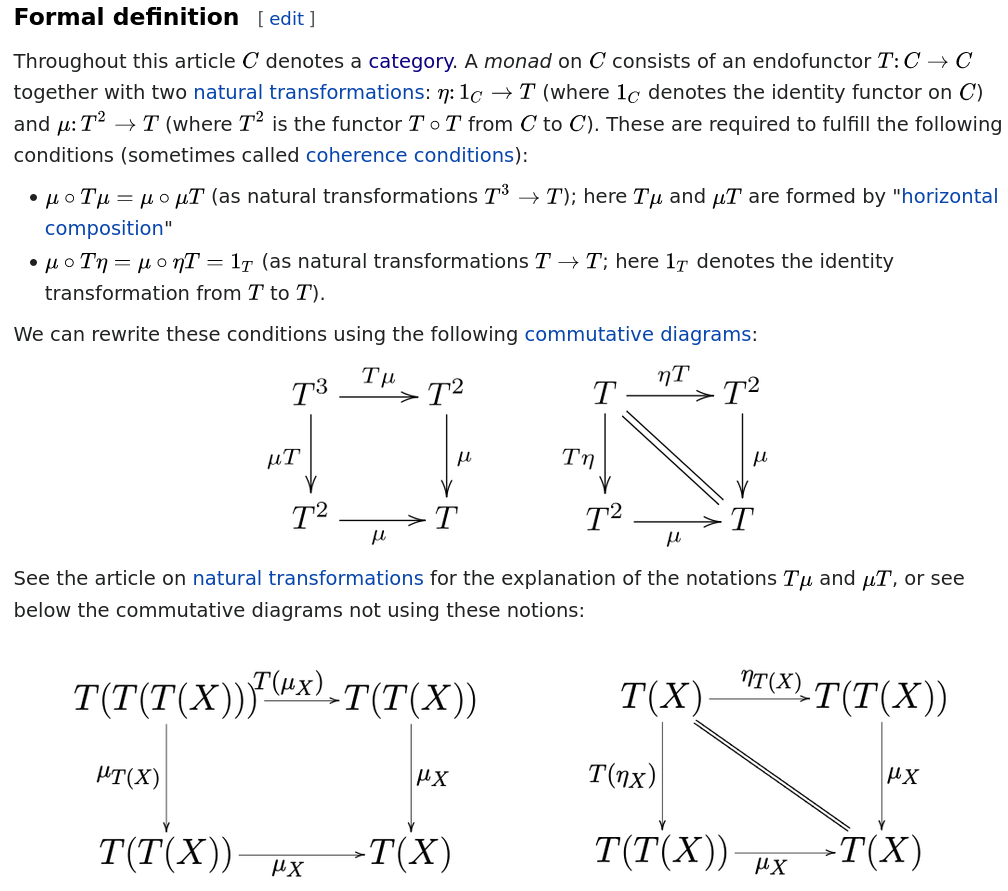
\includegraphics[width=\textwidth, height=\textheight]{MonadFormalDef.png}
\end{frame}

\begin{frame}[fragile]
  \frametitle{Lets try again...}
    \begin{itemize}
      \item A Monad is an algebra\footnote{Technically a Kleisli Triple}.
      \item A Monad is a way to sequence effectful computations.
      \item A Monad is a way to enforce referential transparency and purity.
      \item A Monad is a way to reason about the universe.
    \end{itemize}
\end{frame}

\begin{frame}[fragile]
  \frametitle{Let's start with the Algebra}
  \begin{align*}
    \text{Let } C &= \text{M must also be an Applicative!} \\
    \text{Let } M &= (C, A, F, L) \\
    \text{Let } F &= \{ \\
          &\;\;\; \mu : M(M(A)) \to M(A), \\
          &\;\;\; >>= \;: M(A) \to (A \to M(B)) \to M(B) \} \\
    \text{Let } L &= \{ \\
                  &\;\;\;pureIdLeft : pure(x) >>= f = f(x), \\
                  &\;\;\;pureIdRight : m >>= pure = m, \\
                  &\;\;\;assoc : m >>= (\lambda x.f(x) >>= g) = (m >>= f) >>= g \}
  \end{align*}
\end{frame}

\begin{frame}[fragile]
  \frametitle{Verified Monads}
  \begin{itemize}
    \item Time for the demo.
  \end{itemize}
\end{frame}

\begin{frame}[fragile]
  \frametitle{what about the rest?}
    \begin{itemize}
      \item \sout{A Monad is an algebra.}
      \item A Monad is a way to sequence effectful computations.
      \item A Monad is a way to enforce referential transparency and purity.
      \item A Monad is a way to reason about the universe.
    \end{itemize}
\end{frame}

\begin{frame}[fragile]
\frametitle{References}
\bibliography{references}{}
\end{frame}

\end{document}

